\documentclass[a4paper,10pt]{article}

\usepackage{graphicx}
\usepackage{amsmath}
\usepackage[spanish]{babel}
\usepackage[utf8]{inputenc} % Permite escribir directamente áéíóúñ
\usepackage[hidelinks]{hyperref}
\usepackage{pdfpages}

\title{ \textbf{ 6620. Organizaci\'on de Computadoras\\
Trabajo Pr\'actico 0: \\
Infraestructura B\'asica}}

\author{ Riesgo, Daniela, \textit{Padr\'on Nro. 95557} \\
\texttt{ danielap.riesgo@gmail.com } \\[2.5ex]
Martin, D\'ebora, \textit{Padr\'on Nro. 90934} \\
\texttt{ debbie1new.world@gmail.com } \\[2.5ex]
Constantino, Guillermo, \textit{Padr\'on Nro. 89776} \\
\texttt{ guilleconstantino@gmail.com } \\[2.5ex]
\normalsize{2do. Cuatrimestre de 2014} \\
\normalsize{66.20 Organizaci\'on de Computadoras $-$ Pr\'atica Martes} \\
\normalsize{Facultad de Ingenier\'ia, Universidad de Buenos Aires} \\
}

\date{}

\begin{document}
\maketitle
\thispagestyle{empty} % quita el nmero en la primer pagina
\begin{abstract}
El presente trabajo tiene como objetivo familiarizarse con las herramientas de software que ser\'an usadas en los siguientes trabajos, implementando un programa en lenguaje C, y su correspondiente documentaci\'on, que resuelva el problema planteado, que permita dibujar el conjunto de Mandelbrot y sus vecindades

\end{abstract}

\cleardoublepage
\setcounter{page}{0}
\newpage
\tableofcontents

\newpage
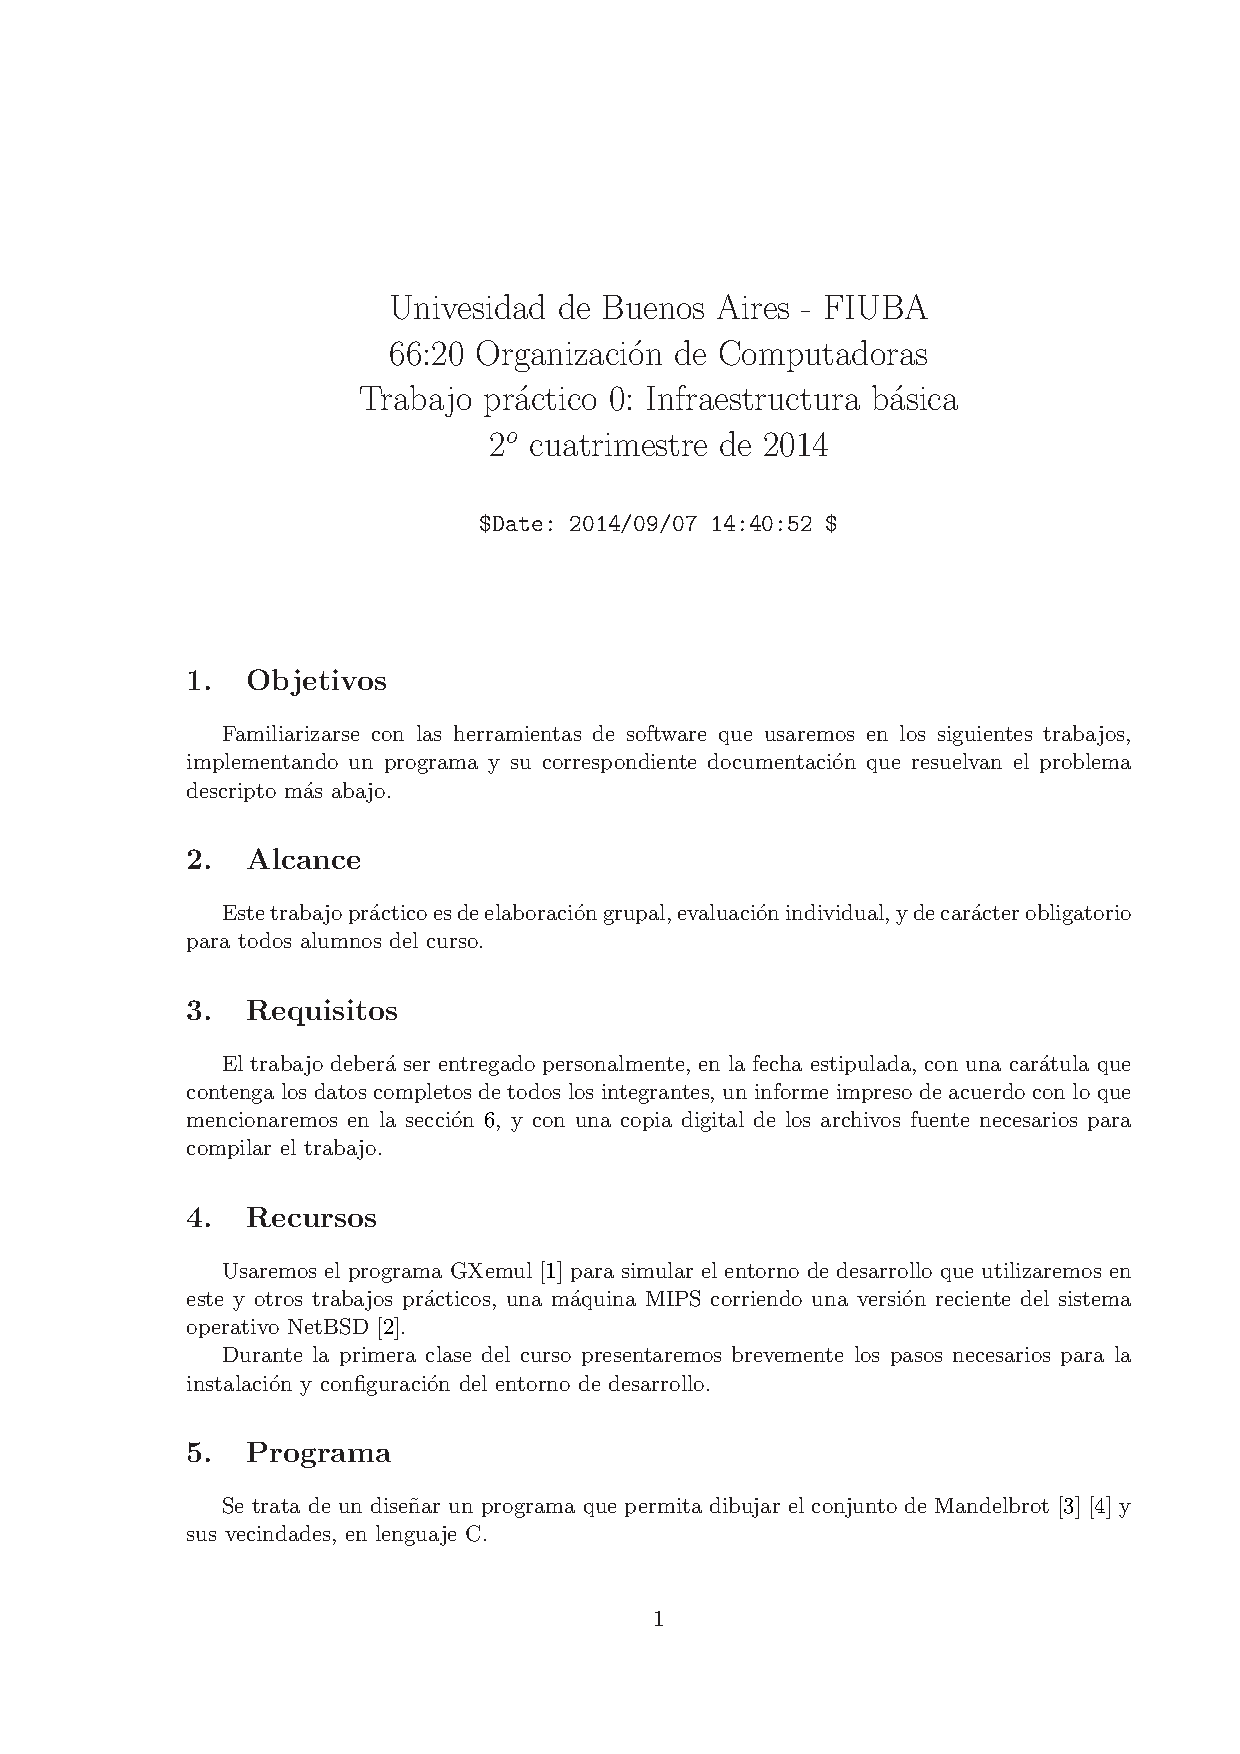
\includepdf[pages={-}, pagecommand={\thispagestyle{empty}}, addtotoc={1, section, 1, Enunciado, enunciado}]{./Enunciado.pdf}
\newpage

\section{Introducci\'on}
Al comenzar a utilizar nuevas herramientas, en cualquier \'ambito, es necesaria una breve introducci\'on al funcionamiento de las mismas: tener una noci\'on de las prestaciones que ofrecen, asi tambi\'en como de sus limitaciones.\\
Como primer objetivo en la materia, nos proponemos adentrarnos en el funcionamiento del emulador GXemul. Nuestra meta ser\'a emular una plataforma MIPS (ejecutando un sistema operativo NetBSD), para poder desde all\'i desarrollar programas en lenguaje C. Estos ser\'an compilados y ejecutados haciendo uso de la herramienta GCC (GNU Compiler Collection), mediante el cual tambi\'en ser\'a posible obtener, a posteriori, el c\'odigo MIPS32 del programa.\\
Una vez cumplido este objetivo, aprenderemos los rudimientos de \LaTeX{} para generar la documentaci\'on relevante al trabajo pr\'actico.




\section{Programa a implementar}
Se trata de un disenar un programa que permita dibujar el conjunto de Mandelbrot y sus vecindades, en lenguaje C.
El mismo recibir\'a por l\'inea de comando, una serie de par\'ametros describiendo la regi\'on del
plano complejo y las caracter\'isticas del archivo imagen a generar. No deber\'a interactuar con
el usuario, ya que no se trata de un programa interactivo, sino m\'as bien de una herramienta
de procesamiento batch. Al finalizar la ejecuci\'on, y volver al sistema operativo, el programa
habr\'a dibujado el fractal en el archivo de salida.
El formato gr\'afico a usar es PGM o portable gray map, un formato simple para describir im\'agenes a
digitales monocrom\'aticas.





\section{Explicaci\'on de la Implementaci\'on}
Las principales funciones y estructuras en nuestra implementaci\'on son las siguientes:

\subsubsection{Main}
Esta funci\'on se encarga de procesar las opciones ingresadas por l\'inea de comando, verificando validez, y luego de resolver los p\'ixeles a tratar y sus números complejos, la velocidad de escape de ellos y la escritura del archivo.

\subsubsection{Generarción del archivo}
Toma un nombre válido de archivo y sabiendo la cantidad de pixeles en filas y columnas, color de gris m\'aximo, y sus valores de color asociados, va escribiendo en el archivo los valores de forma ordenada.

\subsubsection{Velocidad de escape}
Para cada par (parte real, parte imaginaria) que representan a un complejo, calcula su velocidad de escape. Este valor define una intensidad de color seg\'un la condici\'on de corte.


\section{Generaci\'on de ejecutables y c\'odigo assembly}
Para generar el ejecutable del programa, debe correrse la siguiente sentencia en una terminal:

\begin{verbatim}
$ gcc -Wall -pedantic --std=c99 -c velocidad_escape.c
$ gcc -Wall -pedantic --std=c99 -c pgm.c
$ gcc -Wall -pedantic --std=c99 velocidad_escape.o pgm.o \
main.c -o tp0
\end{verbatim}

Para generar el c\'odigo MIPS32, debe ejecutarse lo siguiente:
\begin{verbatim}
$ gcc -Wall -S -pedantic --std=c99 -c velocidad_escape.c
$ gcc -Wall -S -pedantic --std=c99 -c pgm.c
$ gcc -Wall -S -pedantic --std=c99 velocidad_escape.o pgm.o \
main.c -o tp0
\end{verbatim}

N\'otese que para ambos casos se han activado todos los mensajes de 'Warning' (-Wall). Adem\'as, para el caso de MIPS, se ha habilitado '-S', que detiene al compilador luego de generar el assembly.
\pagebreak




\section{Corridas de prueba}

En esta secci\'on se presentan algunas de las distintas corridas que se
realizaron para probar el funcionamiento del trabajo pr\'actico.\\

1. Generamos una imagen de 1 punto de lado, centrada en el or\'igen del plano complejo:
\begin{verbatim}
> ./tp0 -c 0+0i -r 1x1 -o -
P2
1
1
255
255
\end{verbatim}

Notar que el resultado es correcto, ya que este punto pertenece al conjunto de Mandelbrot.\\
\\
2. Repetimos el experimento, pero nos centramos ahora en un punto que seguro no pertenece
al conjunto:
\begin{verbatim}
> ./tp0 -c 10+0i -r 1x1 -o -
P2
1
1
255
0
\end{verbatim}

Notar que el resultado es correcto, ya que este punto pertenece al conjunto de Mandelbrot.
\\
3. Imagen imposible:
\begin{verbatim}
> ./tp0 -c 0+0i -r 0x1 -o -
fatal: invalid resolution specification
Usage:
		tp0 -H, for height of the complex plane (4 by default)
		tp0 -w, for width of the complex plane (4 by default)
		tp0 -r, for resolution of the image: AxB format with A and B natural
		numbers (640x480 by default)
		tp0 -c, for centre of the complex plane: A+Bi format with A and B
		numbers (0+0i by default)
		tp0 -o, for pgm output file (stdout by default)
\end{verbatim}


4. Archivo de salida imposible:
\begin{verbatim}
> ./tp0 -o /tmp
fatal: cannot open output file
Usage:
		tp0 -H, for height of the complex plane (4 by default)
		tp0 -w, for width of the complex plane (4 by default)
		tp0 -r, for resolution of the image: AxB format with A and B natural
		numbers (640x480 by default)
		tp0 -c, for centre of the complex plane: A+Bi format with A and B
		numbers (0+0i by default)
		tp0 -o, for pgm output file (stdout by default)
\end{verbatim}


5. Coordenadas complejas imposibles:
\begin{verbatim}
> ./tp0 -c 1+3 -o -
fatal: invalid center specification
Usage:
		tp0 -H, for height of the complex plane (4 by default)
		tp0 -w, for width of the complex plane (4 by default)
		tp0 -r, for resolution of the image: AxB format with A and B natural
		numbers (640x480 by default)
		tp0 -c, for centre of the complex plane: A+Bi format with A and B
		numbers (0+0i by default)
		tp0 -o, for pgm output file (stdout by default)
\end{verbatim}


6. Argumentos de l\'inea de comando vac\'ios,
\begin{verbatim}
> ./tp0 -c "" -o -
fatal: invalid center specification
Usage:
		tp0 -H, for height of the complex plane (4 by default)
		tp0 -w, for width of the complex plane (4 by default)
		tp0 -r, for resolution of the image: AxB format with A and B natural
		numbers (640x480 by default)
		tp0 -c, for centre of the complex plane: A+Bi format with A and B
		numbers (0+0i by default)
		tp0 -o, for pgm output file (stdout by default)
\end{verbatim}


7. Imagen PGM
\begin{verbatim}
> ./tp0 -o por_default.pgm
\end{verbatim}
Genera la siguiente imagen:
\begin{figure}
\begin{center}

\includegraphics[width=0.8\textwidth]{./por_default.png}
\label{fig:Region barrida por defecto}
\caption{}
\end{center}
\end{figure}


8. Imagen PGM con regi\'on no centrada y un rect\'angulo de 0,005 unidades de lado.
\begin{verbatim}
> ./tp0 -c +0.282-0.01i -w 0.005 -H 0.005 -o zoom.pgm
\end{verbatim}
Genera la siguiente imagen:
\begin{figure}
\begin{center}

\includegraphics[width=0.8\textwidth]{./zoom.png}
\label{fig:Region comprendida entre 0,2795 - 0,0075i y 0,2845 - 0,0125i}
\caption{}
\end{center}
\end{figure}


9. Se puede ver en la sección del código fuente otras pruebas unitarias hechas para probar la función de velocidad de escape en el archivo pruebas\_escape.c.
\begin{verbatim}
> gcc -Wall -pedantic --std=c99 pruebas_escape.c \
-o prueba_escape
> ./prueba_escape
Vel de escape de 0+0i es 255: OK
Vel de escape de 10+0i es 0: OK
Vel de escape de -1+0i es 255: OK
Vel de escape de 0,5+0i es 4: OK
Vel de escape de 1+0i es 2: OK
\end{verbatim}

10. De la misma forma para pruebas unitarias respecto a la lógica del escalamiento de la imagen, se tiene el archivo pruebas\_escala.c.
\begin{verbatim}
> gcc -Wall -pedantic --std=c99 pruebas_escala.c \
-o prueba_escala
> ./prueba_escala
Complejos para -c 0+0i -r 2x2 -w 4 -H 4:
-1.000000 + 1.000000 i
1.000000 + 1.000000 i
-1.000000 + -1.000000 i
1.000000 + -1.000000 i
El primero es correcto: OK
El segundo es correcto: OK
El tercero es correcto: OK
El cuarto es correcto: OK
Complejos para -c 10+0i -r 1x1 -w 4 -H 4:
10.000000 + 0.000000 i
El primero es correcto: OK
Complejos para -c -3.5+1i -r 1x1 -w 4 -H 4:
-3.500000 + 1.000000 i
El primero es correcto: OK
Complejos para -c 1-3i -r 2x1 -w 2 -H 3:
0.500000 + -3.000000 i
1.500000 + -3.000000 i
El primero es correcto: OK
El segundo es correcto: OK
\end{verbatim}



\section{C\'odigo fuente C}

\subsection{main.c}

\begin{verbatim}
#include <stdlib.h>
#include <getopt.h>
#include <stdio.h>
#include <stdbool.h>
#include <string.h>

#define DEFAULT_RESOLUTION_WIDTH 640
#define DEFAULT_RESOLUTION_HEIGHT 480
#define DEFAULT_CENTER_REAL 0
#define DEFAULT_CENTER_IMAG 0
#define DEFAULT_PLANE_WIDTH 4
#define DEFAULT_PLANE_HEIGHT 4
#define DEFAULT_MAX_GRAY 255
#define ARG_DEFAULT_OUT "-"

int main(int argc, char* argv[]){
    static struct option long_options[] =
    {
        {"resolution", required_argument, 0, 'r'},
        {"center", required_argument, 0, 'c'},
        {"width", required_argument, 0, 'w'},
        {"height", required_argument, 0, 'H'},
        {"output", required_argument, 0, 'o'},
        {0, 0, 0, 0}
    };

    int resolution[2];
    float center[2];
    float plane[2];
	int max_gray;
    FILE* output;
	
	// La inicializo por default
	resolution[0] = DEFAULT_RESOLUTION_WIDTH;
    resolution[1] = DEFAULT_RESOLUTION_HEIGHT;
    center[0] = DEFAULT_CENTER_REAL;
    center[1] =  DEFAULT_CENTER_IMAG;
    plane[0] = DEFAULT_PLANE_WIDTH;
    plane[1] = DEFAULT_PLANE_HEIGHT;
	max_gray = DEFAULT_MAX_GRAY;
    output = stdout;
	

	// Parseo y verifico argumentos.
    bool need_close = false;
    char option, i;
    int option_index;

    while ((option = getopt_long(argc, argv, "o:r:c:w:H:", long_options,
    		 &option_index)) != -1) {
        switch (option){
            case 'r':
                if (sscanf(optarg, "%d%*c%d", &resolution[0], 
                	&resolution[1]) != 2){
                    printf("fatal: invalid resolution specification\n");
                    goto usage;
                }
                if (resolution[0] <= 0 || resolution[1] <= 0){
                    printf("fatal: invalid resolution specification\n");
                    goto usage;
                }

                break;
            case 'c':
                if (sscanf(optarg, "%f%*c%f%c", &center[0], &center[1], &i) != 3
                	 || i!='i'){
                    printf("fatal: invalid center specification\n");
                    goto usage;
                }
                break;
            case 'w':
                plane[0] = atof(optarg);
                if (plane[0] <= 0){
                    printf("fatal: invalid width specification\n");
                    goto usage;
                }
                break;
            case 'H':
                plane[1] = atof(optarg);
                if (plane[1] <= 0){
                    printf("fatal: invalid height specification\n");
                    goto usage;
                }
                break;
            case 'o':
                if (strcmp(ARG_DEFAULT_OUT, optarg) != 0){
                    output = fopen(optarg, "w");
                    if (! output){
                        printf("fatal: cannot open output file\n");
                        goto usage;
                    }
                    need_close = true;
                }
                break;
            default:
            usage:
                printf("Usage:\n\ttp0 -H, for height of the complex plane 
                (4 by default)\n
                \ttp0 -w, for width of the complex plane (4 by default)\n
                \ttp0 -r, for resolution of the image: AxB format with A and
                B natural numbers (640x480 by default)\n
                \ttp0 -c, for centre of the complex plane: A+Bi format with
                A and B numbers 
                (0+0i by default)\n
                \ttp0 -o, for pgm output file (stdout by default)\n");
                return 1;
        }
    }
    
	// Calculo y escribo el archivo:
	
	// Armo escala.
	double first_real_value = center[0] - plane[0]/2;
    double first_imaginary_value = center[1] + plane[1]/2;
    double width_scale = (plane[0] / resolution[0]);
    double height_scale =  - (plane[1] / resolution[1]);
    first_real_value += width_scale/2;
    first_imaginary_value += height_scale/2;
	
	// Escribo parámetros de la imagen.
	fprintf(output, "P2\n");
	fprintf(output, "%d\n%d\n", resolution[0], resolution[1]);
	fprintf(output, "%d\n", max_gray);

	// Escribo valor de cada pixel.
	int j, k;
	for (j = 0; j < resolution[1]; ++j){
		for (k = 0; k < resolution[0]; ++k) {
            
			double real = first_real_value + k * width_scale;
			double imag = first_imaginary_value + j * height_scale;
			
			// Calculo velocidad de escape
			int vel;
			for (vel = 0; vel < max_gray; ++vel) {
				if ((real * real + imag * imag) > 4)
					//Módulo al cuadrado > 4
					break;
				// Sino, elevo al cuadrado y le sumo a si mismo
				real = real * real - imag * imag + real;
				imag = 2 * real * imag + imag;
			}
			
			fprintf(output, "%d ", vel);
		}
		fprintf(output, "\n");
	}
	// Terminé de escribir el archivo.
	
	
    if (need_close) fclose(output);
    return 0;
}
\end{verbatim}


\subsection{pruebas\_escala.c}
\begin{verbatim}
#include <stdio.h>

void imprimir_complejos_del_plano(double centro_real, double centro_imag, 
double ancho_plano, double alto_plano, int ancho_res, int alto_res, double* v){
	
	double first_real_value = centro_real - ((float)ancho_plano)/2;
    double first_imaginary_value = centro_imag + ((float)alto_plano)/2;
    double width_scale = (((float) ancho_plano) / ancho_res);
    double height_scale =  - (((float) alto_plano) / alto_res);
    first_real_value += width_scale/2;
    first_imaginary_value += height_scale/2;
    
	int contador = 0;
    for(int i = 0; i < alto_res; i++){
        for(int j = 0; j < ancho_res; j++){
			double real = first_real_value + j * width_scale;
			double imag = first_imaginary_value + i * height_scale;
			
			printf("%f + %f i\n", real, imag);
			
			v[contador] = real;
			contador++;
			v[contador] = imag;
			contador++;
		}
	}

}

int main(){

	printf("Complejos para -c 0+0i -r 2x2 -w 4 -H 4:\n");
    double v1[8];
    imprimir_complejos_del_plano(0, 0, 4, 4, 2, 2, v1);
	printf("El primero es correcto: %s\n", ((v1[0] == -1) & (v1[1] == 1))?
			 "OK" : "ERROR");
	printf("El segundo es correcto: %s\n", ((v1[2] == 1) & (v1[3] == 1))? 
			"OK" : "ERROR");
	printf("El tercero es correcto: %s\n", ((v1[4] == -1) & (v1[5] == -1))?
			 "OK" : "ERROR");
	printf("El cuarto es correcto: %s\n", ((v1[6] == 1) & (v1[7] == -1))? 
			"OK" : "ERROR");
	
	printf("Complejos para -c 10+0i -r 1x1 -w 4 -H 4:\n");
    double v2[2];
    imprimir_complejos_del_plano(10, 0, 4, 4, 1, 1, v2);
	printf("El primero es correcto: %s\n", ((v2[0] == 10) & (v2[1] == 0))?
															 "OK" : "ERROR");
	
	printf("Complejos para -c -3.5+1i -r 1x1 -w 4 -H 4:\n");
    double v3[2];
    imprimir_complejos_del_plano(-3.5, 1, 4, 4, 1, 1, v3);
	printf("El primero es correcto: %s\n", ((v3[0] == - 3.5) & (v3[1] == 1))?
			 "OK" : "ERROR");
	
	printf("Complejos para -c 1-3i -r 2x1 -w 2 -H 3:\n");
    double v4[4];
    imprimir_complejos_del_plano(1, -3, 2, 3, 2, 1, v4);
	printf("El primero es correcto: %s\n", ((v4[0] == 0.5) & (v4[1] == -3))?
			 "OK" : "ERROR");
	printf("El segundo es correcto: %s\n", ((v4[2] == 1.5) & (v4[3] == -3))?
			 "OK" : "ERROR");
	
	return 0;
}
\end{verbatim}


\subsection{pruebas\_escala.c}
\begin{verbatim}
#include <stdio.h>

int main(){
        double real, imag;
        int vel;
        
        real = 0;
        imag = 0;
        
        for (vel = 0; vel < max_gray; ++vel) {
			if ((real * real + imag * imag) > 4)
            //Módulo al cuadrado > 4
				break;
            // Sino, elevo al cuadrado y le sumo a si mismo
            real = real * real - imag * imag + real;
            imag = 2 * real * imag + imag;
        }
        
        printf("%s: %s\n", "Vel de escape de 0+0i es 255", (vel == 255)? 
        		"OK" : "ERROR");

        real = 10;
        imag = 0;
        
        for (vel = 0; vel < max_gray; ++vel) {
			if ((real * real + imag * imag) > 4)
            //Módulo al cuadrado > 4
				break;
            // Sino, elevo al cuadrado y le sumo a si mismo
            real = real * real - imag * imag + real;
            imag = 2 * real * imag + imag;
        }

        printf("%s: %s\n", "Vel de escape de 10+0i es 0", (vel == 0)? 
        		"OK" : "ERROR");
       
        real = -1;
        imag = 0;
        
        for (vel = 0; vel < max_gray; ++vel) {
			if ((real * real + imag * imag) > 4)
            //Módulo al cuadrado > 4
				break;
            // Sino, elevo al cuadrado y le sumo a si mismo
            real = real * real - imag * imag + real;
            imag = 2 * real * imag + imag;
        }

        printf("%s: %s\n", "Vel de escape de -1+0i es 255", (vel == 255)? 
        		"OK" : "ERROR");
       
        real = 0.5;
        imag = 0;
        
        for (vel = 0; vel < max_gray; ++vel) {
			if ((real * real + imag * imag) > 4)
            //Módulo al cuadrado > 4
				break;
            // Sino, elevo al cuadrado y le sumo a si mismo
            real = real * real - imag * imag + real;
            imag = 2 * real * imag + imag;
        }


        printf("%s: %s\n", "Vel de escape de 0,5+0i es 4", (vel == 4)? 
        		"OK" : "ERROR");
       
        real = 1;
        imag = 0;
        
        for (vel = 0; vel < max_gray; ++vel) {
			if ((real * real + imag * imag) > 4)
            //Módulo al cuadrado > 4
				break;
            // Sino, elevo al cuadrado y le sumo a si mismo
            real = real * real - imag * imag + real;
            imag = 2 * real * imag + imag;
        }


        printf("%s: %s\n", "Vel de escape de 1+0i es 2", (vel == 2)? 
        		"OK" : "ERROR");
}

\end{verbatim}

\pagebreak



\section{Conclusiones}
El trabajo pr\'activo motivo de este informe ha presentado al equipo diversos desaf\'ios. En primer lugar cabe mencionar la adaptaci\'on a un ambiente basado en GNU/Linux, no dominado por todos sus integrantes de igual manera. Tambi\'en es destacable la dificultad inicial que trajo la correcta configuraci\'on del ambiente virtual utilizado para emular la m\'aquina MIPS. Finalmente, tambi\'en fue invertida una cantidad considerable de tiempo en aprender a utilizar e investigar sobre archivos PGM y principalmente \LaTeX{}, ya que si bien permite obtener muy buenos resultados, se requiere de mucha lectura para poder aprovechar todo su potencial.
Por las razones expuestas, consideramos muy necesario un trabajo pr\'actico introductorio de esta naturaleza, para nivelar e introducir los elementos a utilizar en las dem\'as actividades pr\'acticas que se desarrollar\'an en el curso.\\
Como conclusi\'on final, podemos considerar que hemos logrado obtener un buen manejo de las herramientas introducidas en este primer proyecto.

\pagebreak

\begin{thebibliography}{99}

\bibitem{GXEMUL} GXemul, \url{http://gxemul.sourceforge.net/}

\bibitem{NETBSD} The NetBSD Project, \url{http://www.netbsd.org/}

\bibitem{MANDEL} Mandelbrot, \url{http://en.wikipedia.org/wiki/Mandelbrot\_set/}

\bibitem{MANSET} Introduction to the Mandelbrot Set,
\url{http://www.olympus.net/personal/dewey/mandelbrot.html}.

\bibitem{MANEXT} Smooth shading for the Mandelbrot exterior.
\url{http://linas.org/art-gallery/escape/smooth.html}. Linas Vepstas. October, 1997.

\bibitem{PGMFORMAT} PGM format specification.
\url{http://netpbm.sourceforge.net/doc/pgm.html}

\bibitem{LATEX} Oetiker, Tobias, "The Not So Short Introduction To LaTeX2", \url{http://www.physics.udel.edu/$\sim$dubois/lshort2e/}

\end{thebibliography}


\end{document}
